%%==================================================================
\section{Profiles, optima and polynomials}\label{sec:applications}
%%==================================================================

This section draws the consequences of Theorem~\ref{thm:weighted} and of
Theorem~\ref{thm:bounded-occ}. The pattern is the same each time: a
combinatorial quantity is written as the sum \eqref{eq:Z} of a factor system
over a cube, the algebra is chosen so that the sum records what one wants to
know, and the two theorems are applied. The only place where something has to
be added to the summation routine is the independence polynomial of a graph
without any bound on the degrees, in Section~\ref{ssec:indep}, where a
branching rule reduces the general graph to graphs of small degree; the cost of
the rule is bounded by an explicit induction.

\subsection{Profiles of sparse constraint systems}\label{ssec:profile}
A \emph{constraint system} on $n$ Boolean variables consists of constraints
$C_1,\dots,C_m$, where $C_f:\{0,1\}^{I_f}\to\{0,1\}$ is given by its truth
table on a scope $I_f\subseteq[n]$, together with nonnegative integer weights
$\omega_1,\dots,\omega_m$. For an assignment $x$ write
\[
  \sat_\omega(x)=\sum_{f:\,C_f(x|_{I_f})=1}\omega_f
\]
for the weight of the constraints it satisfies. The \emph{profile} of the
system is the sequence
\begin{equation}\label{eq:csprofile}
  p_j=\#\{x\in\{0,1\}^n:\sat_\omega(x)=j\},\qquad 0\le j\le\Omega_{\mathrm{tot}}=\sum_f\omega_f .
\end{equation}

\begin{theorem}[Profiles]\label{thm:profile}
Fix integers $k\ge1$ and $c\ge1$. There is a deterministic algorithm that, given
a constraint system on $n\ge20$ variables with $m\le cn$ constraints of scope at
most $k$ and weights $\omega_f\le\Omega$, computes the whole profile
\eqref{eq:csprofile} in time $\poly(n,\Omega)\,2^{O_{k,c}(\rhon(n))}$ and
polynomial space.
\end{theorem}

\begin{proof}
Let $N=1+\Omega_{\mathrm{tot}}\le 1+cn\Omega$ and $\A=\A_N$. For each $f$ let
$\Phi_f$ be the multilinear extension \eqref{eq:multilinear} of the function
$\phi_f(x)=W^{\omega_f C_f(x)}$ on $\{0,1\}^{I_f}$; its coefficients are the
polynomials $\sum_{U\subseteq S}(-1)^{|S|-|U|}\phi_f(\mathbf 1_U)$, each a sum of
at most $2^k$ monomials $\pm W^{j}$, so they are polynomials in $W$ with integer
coefficients of absolute value at most $2^k$. The system $(\Phi_f)$ is a factor
system with at most $cn$ factors of scope at most $k$, and by
\eqref{eq:profile}, since $\sum_f\omega_fC_f(x)=\sat_\omega(x)\le\Omega_{\mathrm{tot}}<N$,
\[
  Z=\sum_{x}\prod_f W^{\omega_fC_f(x|_{I_f})}=\sum_{j}p_jW^{j}
\]
with no term lost to the truncation. Theorem~\ref{thm:weighted} computes $Z$
with $\poly(n)2^{O_{k,c}(\rhon(n))}$ operations in $\A_N$ and factor
evaluations, and Lemma~\ref{lem:bits} with $L=k$ bounds the bit lengths by
$\poly(n,N)$, so the bit cost is $\poly(n,\Omega)2^{O_{k,c}(\rhon(n))}$. The
coefficients $p_j$ are read off from $Z$.
\end{proof}

The profile contains, besides the optimum, every quantity that depends only on
the distribution of the objective over the cube.

\begin{corollary}[Max-$k$-SAT]\label{cor:maxsat}
Fix $k,c\ge1$. Given a $k$-CNF formula with $n$ variables and $m\le cn$ clauses
with integer weights in $[0,\Omega]$, the following are computed deterministically
in time $\poly(n,\Omega)2^{O_{k,c}(\rhon(n))}$: the maximum weight of
simultaneously satisfiable clauses, the number of assignments attaining it, the
minimum such weight, and for every $j$ the number of assignments satisfying
clauses of total weight exactly $j$. In particular Max-$k$-SAT, Min-$k$-SAT and
weighted Max-$k$-SAT with polynomially bounded weights are solved exactly in time
$2^{o(n)}$ on instances with $O(n)$ clauses, and the number of optimal
assignments is counted.
\end{corollary}

\begin{proof}
A clause is a constraint whose truth table is the disjunction of its literals.
Apply Theorem~\ref{thm:profile}; the maximum is the largest $j$ with $p_j>0$,
the minimum the smallest, and $p_j$ is the required count.
\end{proof}

The Hamming weight of an assignment is itself a sum of local weights, one per
variable, so the profile may be taken with respect to it.

\begin{corollary}[Satisfying assignments of each weight]\label{cor:hamming}
Fix $k,c\ge1$. Given a $k$-CNF formula with $n$ variables and $m\le cn$ clauses,
the numbers
\[
  s_i=\#\{x:\ x\text{ satisfies the formula and has exactly $i$ ones}\},\qquad 0\le i\le n,
\]
are computed deterministically in time $\poly(n)2^{O_{k,c}(\rhon(n))}$. Hence the
satisfying assignment with the fewest, or the most, ones is found and counted
within the same time.
\end{corollary}

\begin{proof}
Take $\A=\A_{n+1}$. For each clause $f$ let $\Phi_f$ be the multilinear extension
of its satisfaction indicator, with coefficients in $\{0,\pm1\}\subseteq\Q$, and
for each variable $v$ add the factor $\Phi_v=1+(W-1)Y_v$ of scope $\{v\}$,
the multilinear extension of $W^{x_v}$. The system has at most $(c+1)n$ factors
of scope at most $k$, and its sum is
$Z=\sum_x[\text{$x$ satisfies the formula}]\,W^{|x|}=\sum_is_iW^i$, where $|x|$
is the number of ones. Theorem~\ref{thm:weighted} and Lemma~\ref{lem:bits}
with $N=n+1$, $L=1$ give the time bound. A satisfying assignment of a prescribed
weight $i$ with $s_i>0$ is then found by the usual self-reduction: fix the first
variable to $0$ and to $1$, recompute the profiles of the two restricted
formulas, which are again sparse $k$-CNF formulas, keep a value for which the
coefficient of $W^{i}$ or $W^{i-1}$ is positive, and continue; this multiplies
the time by at most $2n$.
\end{proof}

The next corollary uses an algebra in two variables, one recording the cut and
one the size of a side.

\begin{corollary}[Max-Cut and bisections]\label{cor:maxcut}
Fix $c\ge1$. Given a graph $G$ with $n$ vertices and $m\le cn$ edges with integer
weights in $[0,\Omega]$, the numbers
\[
  q_{i,j}=\#\{S\subseteq V(G):\ |S|=i,\ \text{the edges between $S$ and $V\setminus S$ have total weight $j$}\}
\]
are computed for all $i$ and $j$ in deterministic time
$\poly(n,\Omega)2^{O_c(\rhon(n))}$. In particular the maximum cut, the maximum
and the minimum bisection, with the number of optimal solutions of each, are
computed exactly in time $2^{o(n)}$ on graphs with $O(n)$ edges.
\end{corollary}

\begin{proof}
Let $N_1=1+\sum_e\omega_e\le1+cn\Omega$ and $N_2=n+1$, and let
$\A=\A_{N_1,N_2}=\Q[W,U]/(W^{N_1},U^{N_2})$. Encode $S$ by $x\in\{0,1\}^n$. For an
edge $e=\{u,v\}$ take the multilinear extension of $W^{\omega_e[x_u\ne x_v]}$,
which is $1+(W^{\omega_e}-1)(Y_u+Y_v-2Y_uY_v)$, and for each vertex $v$ the
factor $1+(U-1)Y_v$. There are at most $(c+1)n$ factors of scope at most $2$,
with coefficients that are polynomials in $W$ and $U$ with integer coefficients
of absolute value at most $2$. The sum is
$Z=\sum_x W^{\mathrm{cut}(x)}U^{|x|}=\sum_{i,j}q_{i,j}W^{j}U^{i}$, and no term is
truncated. Theorem~\ref{thm:weighted} and Lemma~\ref{lem:bits} with
$N=N_1N_2$ and $L=1$ give the bound. The maximum cut is the largest $j$ with
$\sum_iq_{i,j}>0$, the maximum bisection the largest $j$ with
$q_{\lfloor n/2\rfloor,j}>0$, the minimum bisection the smallest such $j$, and
the counts are the coefficients.
\end{proof}

\begin{figure}[t]
\centering
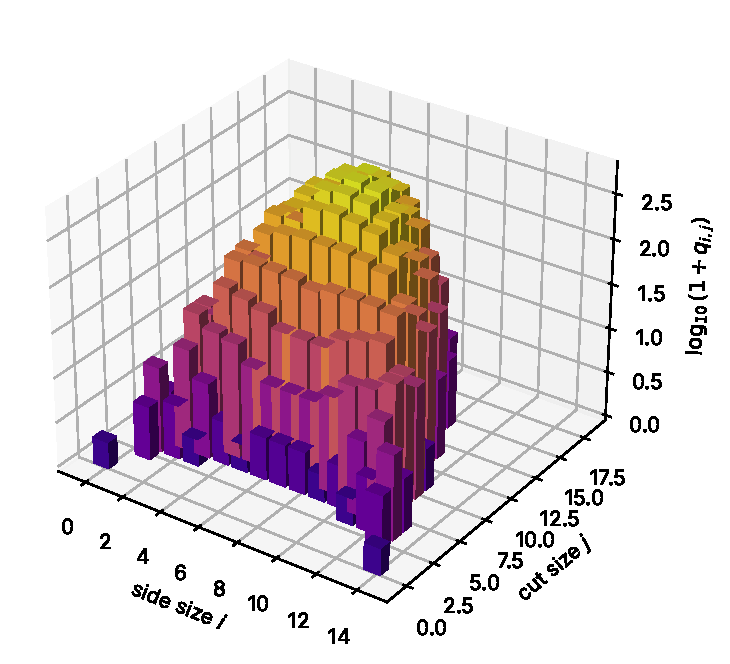
\includegraphics[width=0.74\textwidth]{figures/fig_profile}
\caption{The array $q_{i,j}$ of Corollary~\ref{cor:maxcut} for a graph with
$14$ vertices and $21$ edges, a Hamilton cycle with seven chords, computed
directly from the $2^{14}$ subsets; the height is $\log_{10}(1+q_{i,j})$. The
algorithm returns the whole array as one element of $\Q[W,U]/(W^{22},U^{15})$;
its maximum cut and its maximum bisection are both $18$.}
\label{fig:profile}
\end{figure}

\begin{remark}
The best exact algorithm for Max-Cut on general graphs runs in time
$2^{\omega n/3}\le2^{0.792n}$ \cite{Wil05}, and the exact algorithms for sparse
Max-Cut run in time $2^{\Theta(m)}$ \cite{SS09}; on graphs with $m=O(n)$ edges
both are exponential in $n$. The proof of \oai{}'s Corollary 1.2 contains a
circuit encoding that, combined with their Theorem 1.1, also yields the exact
optimum of a sparse Max-$k$-SAT or Max-Cut instance in time $2^{o(n)}$, by a
binary search over the threshold; that route handles the unweighted objective.
The algebra $\A_N$ handles integer weights up to $\Omega$ at a cost polynomial in
$\Omega$, which a circuit encoding cannot do without introducing $\Theta(n\log\Omega)$
auxiliary variables.
\end{remark}

\subsection{The independence polynomial of every graph}\label{ssec:indep}
Let $G$ be a graph with vertex set $V$, $|V|=n$, and let $\omega:V\to\{0,1,\dots\}$
be integer vertex weights. The weighted independence polynomial is
\begin{equation}\label{eq:indeppoly}
  I_\omega(G;W)=\sum_{S\subseteq V\text{ independent}}W^{\omega(S)},\qquad \omega(S)=\sum_{v\in S}\omega_v ,
\end{equation}
and $I(G;W)=I_{\mathbf 1}(G;W)$ is the independence polynomial. For a vertex $v$
write $N[v]$ for its closed neighbourhood and $G-X$ for the graph induced on
$V\setminus X$. Every independent set either avoids $v$ or contains $v$ and
avoids $N[v]$, so
\begin{equation}\label{eq:indeprec}
  I_\omega(G;W)=I_\omega(G-v;W)+W^{\omega_v}\,I_\omega(G-N[v];W).
\end{equation}

\begin{lemma}[Forcing branching]\label{lem:branch}
Let $b\ge2$ be an integer and $G$ a weighted graph with $n$ vertices. There is a
binary tree, computable in time $\poly(n)$ per node, whose leaves $\ell$ carry
induced subgraphs $H_\ell$ of $G$ of maximum degree at most $b$ and integers
$s_\ell\ge0$ such that
\begin{equation}\label{eq:branchexp}
  I_\omega(G;W)=\sum_{\ell}W^{s_\ell}\,I_\omega(H_\ell;W),
\end{equation}
and the number of leaves is at most
\begin{equation}\label{eq:leaves}
  \Bigl(1+\frac{2\ln(b+2)}{b+1}\Bigr)^{n}.
\end{equation}
\end{lemma}

\begin{proof}
Build the tree from the root $(G,0)$. At a node $(H,s)$ in which some vertex $v$
has degree greater than $b$ in $H$, attach the two children $(H-v,s)$ and
$(H-N_H[v],s+\omega_v)$; by \eqref{eq:indeprec} the sum
$\sum W^{s}I_\omega(H;W)$ over the nodes of any antichain that cuts every
root-to-leaf path is the same, and it equals $I_\omega(G;W)$ at the root. A node
in which every vertex has degree at most $b$ is a leaf. This gives
\eqref{eq:branchexp}, and each node is processed in polynomial time.

Let $L(n)$ be the largest number of leaves of such a tree over all weighted graphs
with at most $n$ vertices, so that $L$ is nondecreasing and $L(n)=1$ for
$n\le b+1$, because a graph with at most $b+1$ vertices has maximum degree at
most $b$. If $v$ has degree at least $b+1$ then $H-v$ has $n-1$ vertices and
$H-N_H[v]$ at most $n-b-2$, so
\[
  L(n)\le L(n-1)+L(n-b-2)\qquad(n\ge b+2),
\]
with $L(j)=1$ for $j\le b+1$, including $j\le0$. Put $\varepsilon=2\ln(b+2)/(b+1)$.
We claim $L(n)\le(1+\varepsilon)^n$ for all $n\ge0$. This holds for $n\le b+1$.
For $n\ge b+2$, by induction,
\[
  L(n)\le(1+\varepsilon)^{n-1}+(1+\varepsilon)^{n-b-2}
  =(1+\varepsilon)^{n-b-2}\bigl((1+\varepsilon)^{b+1}+1\bigr),
\]
and the right side is at most $(1+\varepsilon)^{n}$ exactly when
$\varepsilon(1+\varepsilon)^{b+1}\ge1$. Now $b\ge2$ gives
$2\ln(b+2)\le b+1$, since this holds at $b=2$ ($2\ln4<3$) and the difference
$b+1-2\ln(b+2)$ increases with $b$; so $\varepsilon\le1$, and for
$0\le\varepsilon\le1$ one has $\ln(1+\varepsilon)\ge\varepsilon-\varepsilon^2/2\ge\varepsilon/2$.
Therefore
\[
  (1+\varepsilon)^{b+1}\ge e^{(b+1)\varepsilon/2}=e^{\ln(b+2)}=b+2,
  \qquad
  \varepsilon(1+\varepsilon)^{b+1}\ge\frac{2\ln(b+2)}{b+1}(b+2)\ge2\ln4>1 .
\]
This proves the claim, and \eqref{eq:leaves} follows.
\end{proof}

\begin{figure}[t]
\centering
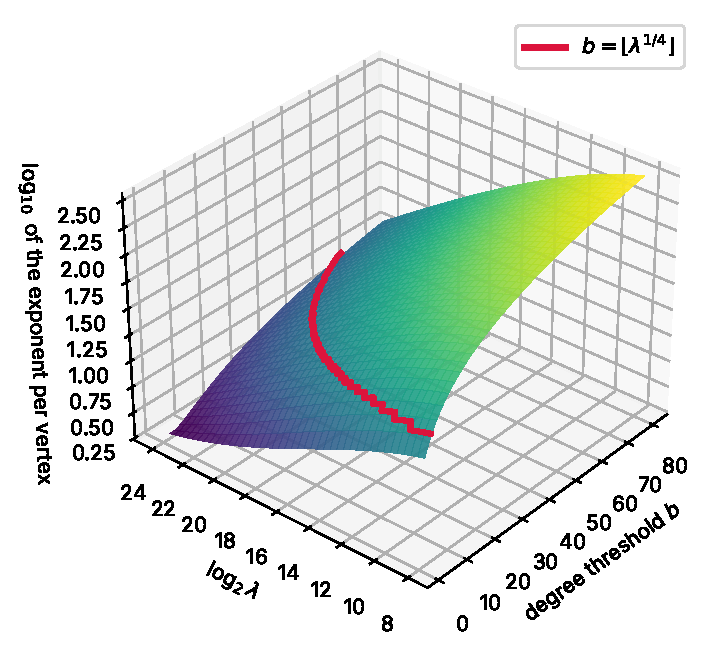
\includegraphics[width=0.78\textwidth]{figures/fig_branch}
\caption{The two costs of the proof of Theorem~\ref{thm:indep} per vertex, in
$\log_{10}$, with the constant $C_0$ omitted: the leaf count
$2\ln(b+2)/(b+1)$ of Lemma~\ref{lem:branch} and the leaf cost
$(b+2)\nu^2/\sqrt\lambda$ of Theorem~\ref{thm:bounded-occ}, as a function of
the degree threshold $b$ and of $\lambda$; the curve marks the choice
$b=\lfloor\lambda^{1/4}\rfloor$ of the proof.}
\label{fig:branch}
\end{figure}

\begin{theorem}[Independence polynomial]\label{thm:indep}
There is a deterministic algorithm that, given a graph $G$ with $n$ vertices and
integer vertex weights in $[0,\Omega]$, computes the weighted independence
polynomial $I_\omega(G;W)$ in time
\[
  \poly(n,\Omega)\,2^{O(n(\log\log n)^2/(\log n)^{1/4})}
\]
and polynomial space. No condition is placed on the graph.
\end{theorem}

\begin{proof}
Let $n_0=n_0(1)$ be the threshold of Theorem~\ref{thm:bounded-occ} with $\beta=1$
and let $n_1\ge n_0^2$ be so large that for $n\ge n_1$ the following hold, with
$\lambda=\lceil\log n\rceil$ and $b=\lfloor\lambda^{1/4}\rfloor$: $b\ge2$,
$\lambda^{1/4}+1\le\lambda/2-1$, and $\lambda/2-1\ge\lambda/3$. For $n<n_1$
compute $I_\omega(G;W)$ by listing the $2^{n}<2^{n_1}$ subsets, a constant. For
$n\ge n_1$ apply Lemma~\ref{lem:branch} with this $b$ and compute
$I_\omega(H_\ell;W)$ at each leaf as follows.

If $H=H_\ell$ has $n_H<\sqrt n$ vertices, list its subsets; this costs
$2^{\sqrt n}\poly(n,\Omega)$. Otherwise $n_H\ge\sqrt n$, so
$\lambda_H=\lceil\log n_H\rceil\ge\lambda/2-1\ge\lambda/3$ and $n_H\ge n_0$. Take
$\A=\A_N$ with $N=1+\sum_v\omega_v\le1+n\Omega$, and the factor system on the
$n_H$ variables $x_v$, $v\in V(H)$, with the factor $1-Y_uY_v$ for each edge
$uv$ of $H$ and the factor $1+(W^{\omega_v}-1)Y_v$ for each vertex $v$. The
edge factor is the multilinear extension of the indicator that $u$ and $v$ are
not both chosen, and the vertex factor that of $W^{\omega_vx_v}$, so the sum
\eqref{eq:Z} is $I_\omega(H;W)$, with no term truncated. Each variable occurs in
at most $\deg_H(v)+1\le b+1\le\lambda^{1/4}+1\le\lambda_H$ factors, the scopes are
at most $2\le\lambda_H$, and the total degree is
$d=2|E(H)|+n_H\le(b+1)n_H$. Theorem~\ref{thm:bounded-occ} with $\beta=1$ and
$\kappa=b+1$ applies and computes $I_\omega(H;W)$ with
\[
  |\F|\,\poly(n_H)\,2^{\,4C_0(b+2)\,n_H\nu_H^2/\sqrt{\lambda_H}}
  \le\poly(n)\,2^{\,4C_0(\lambda^{1/4}+2)\,n\nu^2\sqrt{3/\lambda}}
  =2^{O(n\nu^2/\lambda^{1/4})}
\]
operations in $\A_N$, using $\nu_H\le\nu$ and $\lambda_H\ge\lambda/3$;
Lemma~\ref{lem:bits} with $|\F|\le(b+1)n$, $k=2$, $L=1$ turns this into
$\poly(n,\Omega)2^{O(n\nu^2/\lambda^{1/4})}$ bit operations.

By \eqref{eq:leaves} the tree has at most $(1+\varepsilon)^n\le e^{\varepsilon n}$
leaves with $\varepsilon=2\ln(b+2)/(b+1)\le 4\ln\lambda/\lambda^{1/4}=O(\nu/\lambda^{1/4})$,
hence at most $2^{O(n\nu/\lambda^{1/4})}$ leaves and fewer internal nodes, each
processed in polynomial time, and the leaf polynomials are combined by
\eqref{eq:branchexp} with one multiplication by a power of $W$ and one addition
in $\A_N$ per leaf. The tree is traversed depth first, so only one root-to-leaf
path of length at most $n$ is stored at a time, and the space is polynomial. The
total time is
\[
  2^{O(n\nu/\lambda^{1/4})}\cdot\bigl(2^{\sqrt n}+2^{O(n\nu^2/\lambda^{1/4})}\bigr)\poly(n,\Omega)
  =\poly(n,\Omega)\,2^{O(n\nu^2/\lambda^{1/4})},
\]
and $n\nu^2/\lambda^{1/4}=\Theta(n(\log\log n)^2/(\log n)^{1/4})$.
\end{proof}

\begin{corollary}\label{cor:indep}
Each of the following is computed deterministically, for every graph $G$ on $n$
vertices, in time $2^{O(n(\log\log n)^2/(\log n)^{1/4})}$: the independence
number $\alpha(G)$ and the number of maximum independent sets; the number of
independent sets of each size, hence the partition function of the hard-core
model at every activity; the clique number $\omega(G)$ and the number of maximum
cliques; the vertex cover number $\tau(G)$ and the number of minimum vertex
covers; and, for integer weights in $[0,\Omega]$, the maximum weight of an
independent set and the number of independent sets of that weight, with a factor
$\poly(\Omega)$ in the time.
\end{corollary}

\begin{proof}
$\alpha(G)$ is the degree of $I(G;W)$, its leading coefficient counts the maximum
independent sets, and the coefficient of $W^{i}$ counts the independent sets of
size $i$; the hard-core partition function at activity $z$ is $I(G;z)$. The
cliques of $G$ are the independent sets of the complement, to which
Theorem~\ref{thm:indep} applies without restriction. The vertex covers are the
complements of the independent sets, so $\tau(G)=n-\alpha(G)$ and the minimum
vertex covers are counted by the same leading coefficient. The weighted
statements read the degree and the leading coefficient of $I_\omega(G;W)$.
\end{proof}

\begin{remark}\label{rem:indep}
The fastest published exact algorithm for the maximum independent set runs in
time $2^{0.1996n}$ \cite{XN17}, and $2^{\Omega(n)}$ was a known consequence of
the exponential time hypothesis. \oai{}'s Corollary 1.3 gives the number of
independent sets of every graph in time $2^{o(n)}$ through their Theorem 1.1 in
its general form, which handles formulas with $\Theta(n^2)$ clauses; that form,
combined with a linear-size threshold circuit for the number of chosen vertices,
also gives $\alpha(G)$ with the exponent $n\log\log n/\sqrt{\log n}$. The route
of Theorem~\ref{thm:indep} is different: it uses only the sparse routine
reproduced in Sections \ref{sec:routine} and \ref{sec:design}, reaches every
graph through the branching of Lemma~\ref{lem:branch}, and returns the whole
weighted polynomial. Its exponent is larger, by the factor
$(\log n)^{1/4}\log\log n$, which is the price of the branching.
\end{remark}

The branching of Lemma~\ref{lem:branch} records the weight of the chosen
vertices only through the monomial $W^{\omega_v}$ that multiplies the second
child, and its proof uses nothing else about that monomial. Several weights can
therefore be carried at once, with one generator for each, and a budget can be
placed on each of them. No restriction is placed on the graph.

\begin{theorem}[Independent sets under budgets]\label{thm:indepbudget}
Fix $s\ge0$. There is a deterministic algorithm that, given a graph $G$ with $n$
vertices and weight vectors $\omega^{(0)},\dots,\omega^{(s)}\in\{0,1,\dots,\Omega\}^{V}$,
computes the numbers
\[
  a(j_0,\dots,j_s)=\#\bigl\{S\subseteq V\text{ independent}:\ \omega^{(i)}(S)=j_i\ (0\le i\le s)\bigr\}
\]
for all tuples $(j_0,\dots,j_s)$ in time
\[
  \poly\bigl(n,(1+n\Omega)^{s+1}\bigr)\,2^{O(n(\log\log n)^2/(\log n)^{1/4})}
\]
and polynomial space, the implied constant depending only on $s$.
\end{theorem}

\begin{proof}
Put $N_i=1+\sum_v\omega^{(i)}_v\le1+n\Omega$ and $\A=\A_{N_0,\dots,N_s}$, of
dimension $N=N_0\cdots N_s\le(1+n\Omega)^{s+1}$, and for a vertex $v$ write
$\mathbf W^{v}=\prod_{i=0}^{s}W_i^{\omega^{(i)}_v}$, a basis monomial of $\A$ since
$\omega^{(i)}_v<N_i$. The
polynomial
\[
  I(G)=\sum_{S\text{ independent}}\ \prod_{v\in S}\mathbf W^{v}
  =\sum_{(j_0,\dots,j_s)}a(j_0,\dots,j_s)\,W_0^{j_0}\cdots W_s^{j_s}
\]
loses no term to the truncation, because $\omega^{(i)}(S)<N_i$ for every $S$.
It satisfies $I(G)=I(G-v)+\mathbf W^{v}\,I(G-N[v])$ for every vertex $v$, by the
argument for \eqref{eq:indeprec}. The construction of the tree in
Lemma~\ref{lem:branch} uses only this recursion, with the second child carrying
the product of the monomials $\mathbf W^{v}$ of the vertices fixed to $1$ on the
way, and the bound \eqref{eq:leaves} on the number of leaves uses only the
numbers of vertices removed. So the lemma holds verbatim for $I(G)$, with leaf
terms $\mathbf m_\ell\,I(H_\ell)$ in which $\mathbf m_\ell$ is a monomial.

At a leaf $H=H_\ell$ with $n_H\ge\sqrt n$ vertices take, as in the proof of
Theorem~\ref{thm:indep}, the factor $1-Y_uY_v$ for each edge $uv$ of $H$ and
the factor $1+(\mathbf W^{v}-1)Y_v$ for each vertex $v$, the multilinear
extension of $\prod_i W_i^{\omega^{(i)}_vx_v}$. The sum \eqref{eq:Z} of this
system is $I(H)$. The occurrence numbers, the scopes and the total degree are
those of the proof of Theorem~\ref{thm:indep}, since only the coefficient of
$Y_v$ in the vertex factors has changed, and that coefficient is a polynomial
in the generators with integer coefficients of absolute value at most $1$.
Theorem~\ref{thm:bounded-occ} with $\beta=1$ and $\kappa=b+1$ gives
$\poly(n)2^{O(n\nu^2/\lambda^{1/4})}$ operations in $\A$, and
Lemma~\ref{lem:bits} with $L=1$ turns them into
$\poly(n,N)2^{O(n\nu^2/\lambda^{1/4})}$ bit operations. Leaves with fewer than
$\sqrt n$ vertices are summed directly, each of the at most $2^{\sqrt n}$
subsets costing $\poly(n,N)$. The count of leaves, the depth-first traversal
and the final estimate are those of the proof of Theorem~\ref{thm:indep}, with
$\poly(n,\Omega)$ replaced by $\poly(n,N)$.
\end{proof}

The knapsack problem with a conflict graph \cite{PS09} asks for a set of items
of largest value whose total weight is within a capacity and which contains no
two items joined by an edge of a given graph. It contains the maximum
independent set, and with several capacities it contains the multidimensional
knapsack problem.

\begin{corollary}[Knapsack with an arbitrary conflict graph]\label{cor:knapsack}
Fix $s\ge1$. Given a graph $G$ on $n$ vertices, values $\omega^{(0)}_v$ and
weights $\omega^{(1)}_v,\dots,\omega^{(s)}_v$ in $[0,\Omega]$, and capacities
$B_1,\dots,B_s$, the largest value $\omega^{(0)}(S)$ of an independent set $S$
of $G$ with $\omega^{(i)}(S)\le B_i$ for $1\le i\le s$, and the number of
independent sets attaining it, are computed deterministically in time
$\poly(n,\Omega^{s+1})\,2^{O(n(\log\log n)^2/(\log n)^{1/4})}$. The same holds
with any of the inequalities replaced by equalities or by lower bounds, and
with independent sets replaced by cliques.
\end{corollary}

\begin{proof}
By Theorem~\ref{thm:indepbudget} compute all $a(j_0,\dots,j_s)$. The optimum is
the largest $j_0$ for which $\sum a(j_0,j_1,\dots,j_s)>0$, the sum taken over
the tuples with $j_i\le B_i$ for $1\le i\le s$, and that sum is the number of
optimal sets; it has at most $(1+n\Omega)^{s}$ terms. Other relations between
$j_i$ and $B_i$ change only the range of the sum. Cliques of $G$ are the
independent sets of its complement.
\end{proof}

\subsection{Vertex Cover in time $2^{o(k)}$}\label{ssec:vc}
The parameterised Vertex Cover problem asks, for a graph $G$ with $n$ vertices
and an integer $k$, whether $G$ has a vertex cover with at most $k$ vertices.
We use the kernel of Chen, Kanj and Jia \cite{CKJ01}, which rests on the theorem
of Nemhauser and Trotter \cite{NT75} on the half-integral relaxation of the
problem.

\begin{theorem}[Nemhauser and Trotter; Chen, Kanj and Jia]\label{thm:kernel}
There is a polynomial-time algorithm that, given a graph $G$ and an integer
$k\ge0$, either reports correctly that $G$ has no vertex cover with at most
$k$ vertices, or returns an induced subgraph $G'$ of $G$ with at most $2k$
vertices and an integer $k'\le k$ such that $G$ has a vertex cover with at most
$k$ vertices if and only if $G'$ has one with at most $k'$ vertices.\footnote{In
\cite{CKJ01} the running time is $O(kn+k^3)$; the half-integral optimum is
found by a bipartite matching in the double cover of $G$, and the theorem of
\cite{NT75} says that the vertices valued $1$ lie in some minimum vertex cover
while those valued $0$ lie outside it, so that only the vertices valued $1/2$,
at most $2k$ of them when a cover of size $k$ exists, remain.}
\end{theorem}

\begin{theorem}[Vertex Cover]\label{thm:vc}
Parameterised Vertex Cover is decided deterministically in time
\[
  2^{O(k(\log\log k)^2/(\log k)^{1/4})}+\poly(n),
\]
and the number of vertex covers of $G'$ of each size is obtained within the
same time.
\end{theorem}

\begin{proof}
Run the algorithm of Theorem~\ref{thm:kernel}. If it reports that no cover of
size $k$ exists, answer no. Otherwise it returns $G'$ on $n'\le2k$ vertices and
$k'$. Apply Theorem~\ref{thm:indep} to $G'$ with unit weights and read
$\tau(G')=n'-\alpha(G')$ by Corollary~\ref{cor:indep}; answer yes if and only if
$\tau(G')\le k'$. The time of the second step is
$2^{O(n'(\log\log n')^2/(\log n')^{1/4})}$ with $n'\le2k$, which is
$2^{O(k(\log\log k)^2/(\log k)^{1/4})}$, and the first step is polynomial in $n$.
\end{proof}

\begin{remark}
Under the exponential time hypothesis, Vertex Cover has no algorithm with
running time $2^{o(k)}\poly(n)$ \cite[Theorem 14.6]{CFKLMPPS15}; the hypothesis
being false, the bound of Theorem~\ref{thm:vc} is the first of this shape. The
same kernel argument applies to every parameterised problem with a kernel of
$O(k)$ vertices whose solution is read from an independence polynomial, but we
state no further instance.
\end{remark}

\subsection{Finite domains, homomorphisms and graphical models}\label{ssec:domain}
Variables with more than two values are encoded by blocks of Boolean
variables, one block per variable, and the blocks are kept on the unit vectors
by one factor each. The construction is used for Potts systems below; we
record it in general, since it turns every sparse constraint system over a
fixed finite domain into one over $\{0,1\}$.

\begin{theorem}[Finite domains]\label{thm:domain}
Fix integers $D\ge2$, $k\ge1$ and $c\ge1$. Let $n\ge20$ variables take values
in $[D]$, and let $\F$ be a set of at most $cn$ factors, each a function
$\phi_f:[D]^{I_f}\to\A$ with $|I_f|\le k$, given by its table of $D^{|I_f|}$
values, where $\A$ is $\Q$ or one of the algebras of Lemma~\ref{lem:bits} of
dimension $N$ and the table entries are polynomials in the generators with
integer coefficients of at most $L$ bits. Then
\[
  Z=\sum_{\sigma\in[D]^n}\prod_{f\in\F}\phi_f(\sigma|_{I_f})
\]
is computed deterministically in time $\poly(n,N,L)\,2^{O_{D,k,c}(\rhon(n))}$ and
polynomial space.
\end{theorem}

\begin{proof}
Introduce the $Dn$ Boolean variables $x_{v,a}=[\sigma_v=a]$. For each $v$ let
$\chi_v$ be the indicator on $\{0,1\}^{D}$ that exactly one of
$x_{v,1},\dots,x_{v,D}$ equals $1$, and for each $f$ let $\tilde\phi_f$ be the
function on $\{0,1\}^{D|I_f|}$ that equals $\phi_f(\sigma|_{I_f})$ when every
block of its input is a unit vector, encoding $\sigma|_{I_f}$, and $0$
otherwise. Take as factors the multilinear extensions of the $n$ functions
$\chi_v$, of scope $D$, and of the at most $cn$ functions $\tilde\phi_f$, of
scope at most $kD$. The product of the $\chi_v$ vanishes unless $x$ encodes some
$\sigma\in[D]^n$, and then the product of all factors is
$\prod_f\phi_f(\sigma|_{I_f})$; so the sum \eqref{eq:Z} of this system is $Z$.
The system has $n'=Dn$ variables, at most $(c+1)n\le(c+1)n'$ factors of scope
at most $kD$, and coefficients of at most $L+kD$ bits, since a coefficient of
a multilinear extension is a signed sum of at most $2^{kD}$ table entries.
Theorem~\ref{thm:weighted} with the constants $kD$ and $c+1$ and
Lemma~\ref{lem:bits} give time $\poly(n,N,L)2^{O_{D,k,c}(\rhon(Dn))}$, and
$\rhon(Dn)\le4D\rhon(n)$ for $n\ge D$.
\end{proof}

\begin{corollary}[Homomorphisms and partition functions]\label{cor:hom}
Fix $\Delta\ge1$ and $q\ge1$. Let $A$ be a symmetric $q\times q$ matrix and
$\beta$ a vector of length $q$, both with rational entries of at most $L$ bits.
For a graph $G$ with $n$ vertices and maximum degree $\Delta$, the partition
function
\[
  Z_{A,\beta}(G)=\sum_{\sigma:V(G)\to[q]}\ \prod_{uv\in E(G)}A_{\sigma_u\sigma_v}\prod_{v\in V(G)}\beta_{\sigma_v}
\]
is computed deterministically in time $\poly(n,L)2^{O_{\Delta,q}(\rhon(n))}$. In
particular the number of homomorphisms from $G$ to a fixed graph $H$ on $q$
vertices, with loops allowed, is computed within that time, and so is the
number of proper $q$-colourings of $G$.
\end{corollary}

\begin{proof}
Apply Theorem~\ref{thm:domain} with $D=q$, $\A=\Q$, a factor of scope $\{u,v\}$
with table $A_{ab}$ for each edge and a factor of scope $\{v\}$ with table
$\beta_a$ for each vertex: at most $\Delta n/2+n$ factors of scope at most
$2$. Homomorphisms to $H$ are counted by the adjacency matrix of $H$ and
$\beta=\mathbf 1$; proper colourings by $H=K_q$.
\end{proof}

\begin{remark}
Dyer and Greenhill \cite{DG00} and Bulatov and Grohe \cite{BG05} showed that
$Z_{A}(G)$ is $\#$P-hard for every symmetric nonnegative $A$ outside an
explicit family of matrices of rank at most two in each block; on
bounded-degree graphs every such partition function is now computed exactly in
time $2^{o(n)}$. The same holds for the partition function of any discrete
graphical model whose factors involve a bounded number of variables of bounded
domain and whose factor count is linear: Theorem~\ref{thm:domain} computes it,
and the marginal probability that a variable takes a value is the quotient of
two such sums, the numerator with one indicator factor added.
\end{remark}

\subsection{Spin systems on bounded-degree graphs}\label{ssec:spin}
Let $G$ be a graph with $n$ vertices and maximum degree $\Delta$. An Ising
system on $G$ is given by integer couplings $J_{uv}$ on the edges and integer
fields $h_v$ on the vertices; a configuration is $\sigma\in\{-1,1\}^{V}$ and its
energy is
\begin{equation}\label{eq:ising}
  E(\sigma)=-\sum_{uv\in E(G)}J_{uv}\sigma_u\sigma_v-\sum_{v}h_v\sigma_v .
\end{equation}
The \emph{density of states} is the function $g(E)=\#\{\sigma:E(\sigma)=E\}$, and
the partition function at inverse temperature $\beta$ is
$\mathcal Z(\beta)=\sum_\sigma e^{-\beta E(\sigma)}=\sum_Eg(E)e^{-\beta E}$. Put
$E_{\max}=\sum_{uv}|J_{uv}|+\sum_v|h_v|$, so that $|E(\sigma)|\le E_{\max}$.

\begin{theorem}[Ising and Potts density of states]\label{thm:ising}
Fix $\Delta\ge1$ and $q\ge2$.
\begin{enumerate}[label=(\roman*),leftmargin=2.2em]
\item\label{it:isingmodel} The density of states of an Ising system on a graph of
maximum degree $\Delta$ with $n$ vertices is computed deterministically in time
$\poly(n,E_{\max})2^{O_\Delta(\rhon(n))}$.
\item\label{it:potts} For the $q$-state Potts system with energy
$E(\sigma)=-\sum_{uv}J_{uv}[\sigma_u=\sigma_v]-\sum_vh_v(\sigma_v)$,
$\sigma\in[q]^V$, with integer couplings and integer fields $h_v:[q]\to\Z$, the
density of states is computed in time $\poly(n,E_{\max})2^{O_{\Delta,q}(\rhon(n))}$,
where now $E_{\max}=\sum|J_{uv}|+\sum_v\max_s|h_v(s)|$.
\end{enumerate}
In both cases the ground-state energy and its degeneracy, and the partition
function at every inverse temperature as the finite sum $\sum_Eg(E)e^{-\beta E}$,
follow at once.
\end{theorem}

\begin{proof}
\ref{it:isingmodel} Encode $\sigma_v=(-1)^{x_v}$ with $x\in\{0,1\}^n$. The shifted
energy $E(\sigma)+E_{\max}$ is an integer in $[0,2E_{\max}]$ and is the sum of the
local terms $|J_{uv}|-J_{uv}\sigma_u\sigma_v\in\{0,2|J_{uv}|\}$ over the edges
and $|h_v|-h_v\sigma_v\in\{0,2|h_v|\}$ over the vertices, each nonnegative.
Take $\A=\A_N$ with $N=2E_{\max}+1$ and the factor system consisting of the
multilinear extension of $W^{|J_{uv}|-J_{uv}\sigma_u\sigma_v}$ on the scope
$\{u,v\}$ for each edge and of $W^{|h_v|-h_v\sigma_v}$ on $\{v\}$ for each
vertex. There are at most $\Delta n/2+n$ factors of scope at most $2$, with
coefficients that are polynomials in $W$ with integer coefficients of absolute
value at most $4$, and the sum is $\sum_\sigma W^{E(\sigma)+E_{\max}}=\sum_Eg(E)W^{E+E_{\max}}$.
Theorem~\ref{thm:weighted} with $k=2$, $c=\Delta/2+1$ and Lemma~\ref{lem:bits}
with $L=2$ give the bound.

\ref{it:potts} This is an instance of Theorem~\ref{thm:domain}; we write out the encoding. Encode $\sigma_v\in[q]$ by the $q$ Boolean variables
$x_{v,s}=[\sigma_v=s]$, so that there are $qn$ variables, and let
$\phi_v(x_{v,1},\dots,x_{v,q})$ be the indicator that exactly one of them is $1$,
multiplied by $W^{\max_t|h_v(t)|-h_v(s)}$ for that $s$; this is a function on
$\{0,1\}^{q}$ with values in $\{0\}\cup\{W^{j}:0\le j\le2\max_t|h_v(t)|\}$. For an
edge $uv$ let $\phi_{uv}$ be the function on $\{0,1\}^{2q}$ that equals
$W^{|J_{uv}|-J_{uv}}$ when the two blocks are equal unit vectors, $W^{|J_{uv}|}$
when they are distinct unit vectors, and $1$ otherwise. Take $\A=\A_N$ with
$N=2E_{\max}+1$ and the multilinear extensions of these functions as factors:
$n$ of scope $q$ and at most $\Delta n/2$ of scope $2q$, with coefficients of
absolute value at most $2^{2q}$. The product of the vertex factors vanishes
unless every block is a unit vector, in which case $x$ encodes a configuration
$\sigma$ and the product of all factors is $W^{E(\sigma)+E_{\max}}$. So the sum
is $\sum_Eg(E)W^{E+E_{\max}}$. Theorem~\ref{thm:weighted} on $n'=qn$ variables
with $k=2q$, $c=\Delta/2+1$ and Lemma~\ref{lem:bits} with $L=2q$ give time
$\poly(n,E_{\max})2^{O_{\Delta,q}(\rhon(qn))}$, and
$\rhon(qn)\le q\,n(\log\log n+1)^2/\sqrt{\log n}\le4q\,\rhon(n)$ for
$n\ge q$.
\end{proof}

\begin{remark}
The ground state of an Ising spin glass with couplings in $\{-1,0,1\}$ on a
planar graph with a field, or on a cubic lattice, is NP-hard to find
\cite{Barahona82}, and its density of states is $\#$P-hard to compute, while the partition function of the ferromagnetic model admits a polynomial-time randomised approximation \cite{JS93}; for
bounded-degree graphs Theorem~\ref{thm:ising} computes both in time $2^{o(n)}$
whenever the couplings are polynomially bounded. The $q$-colourings of a graph
are the ground states of the antiferromagnetic Potts system with all $J_{uv}=-1$
and no field, at energy $E=0$; their number for every graph is already in
\oai{}'s Corollary 1.3, and \ref{it:potts} adds the whole density of states on
bounded-degree graphs.
\end{remark}

\subsection{Bounded-degree graphs and sparse set systems}\label{ssec:bounded}
\begin{theorem}\label{thm:bounded}
Fix $\Delta\ge1$, $k\ge1$ and $c\ge1$. Each of the following is computed
deterministically in time $\poly(n,\Omega)2^{O_{\Delta,k,c}(\rhon(n))}$.
\begin{enumerate}[label=(\roman*),leftmargin=2.2em]
\item\label{it:dom} For a graph with $n$ vertices and maximum degree $\Delta$,
with integer vertex weights in $[0,\Omega]$: the number of dominating sets of each
weight, hence the minimum weight of a dominating set and the number of minimum
dominating sets.
\item\label{it:match} For a graph with $n$ vertices and maximum degree $\Delta$,
with integer edge weights in $[0,\Omega]$: the number of matchings of each weight,
hence the matching polynomial, the maximum weight of a matching, the number of
maximum matchings and the number of perfect matchings.
\item\label{it:hit} For a set system of $m\le cn$ sets of size at most $k$ on $n$
elements with integer element weights in $[0,\Omega]$: the number of hitting
sets of each weight, hence the minimum hitting set; and the number of
$2$-colourings of the elements under which exactly $j$ sets are not
monochromatic, for every $j$, hence the maximum number of sets split by a
$2$-colouring.
\end{enumerate}
\end{theorem}

\begin{proof}
\ref{it:dom} Variables $x_v=[v\in S]$. For each vertex $v$ take the multilinear
extension of the function on the scope $N[v]$ that equals $W^{\omega_vx_v}$ if
some $x_u$, $u\in N[v]$, is $1$ and $0$ otherwise; it vanishes unless $S$
dominates $v$. There are $n$ factors of scope at most $\Delta+1$, the sum is
$\sum_{S\text{ dominating}}W^{\omega(S)}$, and Theorem~\ref{thm:weighted} with
$k=\Delta+1$, $c=1$, $N=1+n\Omega$, $L=\Delta+1$ applies.

\ref{it:match} Discard isolated vertices, so that $n\le2m$ where $m\le\Delta n/2$
is the number of edges. Variables $y_e=[e\in M]$, one per edge. For each vertex
$v$ take the multilinear extension of the indicator, on the scope of the edges at
$v$, that at most one of them is chosen; for each edge the factor
$1+(W^{\omega_e}-1)Y_e$. There are $n+m\le3m$ factors of scope at most
$\Delta$ on $m$ variables, the sum is $\sum_{M\text{ matching}}W^{\omega(M)}$,
and Theorem~\ref{thm:weighted} on $m$ variables with $k=\Delta$, $c=3$ applies;
$\rhon(m)\le\rhon(\Delta n/2)=O_\Delta(\rhon(n))$. The coefficient of $W^{n/2}$
for unit weights counts the perfect matchings.

\ref{it:hit} Variables $x_v=[v\in S]$. For the hitting sets, take for each set
$A$ the multilinear extension of the indicator that some $x_v$, $v\in A$, is
$1$, and for each element the factor $1+(W^{\omega_v}-1)Y_v$: at most
$(c+1)n$ factors of scope at most $k$. For the splittings, take for each set
$A$ the multilinear extension of $W^{[\text{$x|_A$ is not constant}]}$, $m\le cn$
factors of scope at most $k$, with $N=m+1$. In both cases
Theorem~\ref{thm:weighted} and Lemma~\ref{lem:bits} with $L=k$ give the bound.
\end{proof}

The permanent of a sparse matrix is a weighted count of perfect matchings in
which the weights multiply rather than add; it needs no truncated algebra at
all.

\begin{theorem}[Sparse permanents]\label{thm:permanent}
Fix $\Delta\ge1$. The permanent of an $n\times n$ integer matrix with at most
$\Delta$ nonzero entries in every row and every column, with entries of absolute
value at most $2^{L}$, is computed deterministically in time
$\poly(n,L)2^{O_\Delta(\rhon(n))}$.
\end{theorem}

\begin{proof}
Let $B$ be the bipartite graph on the rows and columns with an edge $e=(i,j)$ for
each nonzero entry $a_{ij}$; it has $n'\le\Delta n$ edges, and
$\operatorname{per}(A)=\sum_{M}\prod_{e\in M}a_e$ over the perfect matchings $M$
of $B$. If some row or column has no entry the permanent is $0$; otherwise
$n'\ge n$. Take $\A=\Q$, one variable $y_e$ per edge, for each of the $2n$
vertices the multilinear extension of the indicator that exactly one incident
edge is chosen, of scope at most $\Delta$, and for each edge the factor
$1+(a_e-1)Y_e$. There are $2n+n'\le3n'$ factors on $n'$ variables, every
coefficient is an integer of at most $L+1$ bits, and the sum \eqref{eq:Z} is
$\operatorname{per}(A)$. Theorem~\ref{thm:weighted} with $k=\Delta$, $c=3$ and
Lemma~\ref{lem:bits} with $N=1$ give the bound, and
$\rhon(n')=O_\Delta(\rhon(n))$.
\end{proof}

\begin{remark}
The permanent of a $0$-$1$ matrix is $\#$P-complete \cite{Val79}, and for
sparse matrices the best bound known was $2^{n-\Omega(n/\Delta)}$
\cite{CP15}. \oai{}'s Corollary 1.3 counts the perfect matchings of every graph
in time $2^{o(v+e)}$ by their general theorem; Theorem~\ref{thm:permanent}
is the sparse weighted version, with the weights absorbed into the factors over
$\Q$.
\end{remark}

\subsection{One global side constraint}\label{ssec:global}
The factors of a factor system are local, but the algebra may carry one global
statistic for free. Corollary~\ref{cor:hamming} used this for the Hamming weight.
The group algebra of a cyclic group records a residue.

\begin{proposition}[Counting under a congruence]\label{prop:modular}
Fix $k,c\ge1$. Given a $k$-CNF formula with $n$ variables and $m\le cn$ clauses,
integer weights $\omega_v\in[0,\Omega]$ on the variables and a modulus $M\ge1$, the
numbers
\[
  r_j=\#\Bigl\{x:\ x\text{ satisfies the formula and }\sum_v\omega_vx_v\equiv j\pmod M\Bigr\},\qquad 0\le j<M,
\]
are computed deterministically in time $\poly(n,M,\log\Omega)2^{O_{k,c}(\rhon(n))}$.
\end{proposition}

\begin{proof}
Take $\A=\Q[W]/(W^{M}-1)$, the clause indicators as factors, and for each
variable the factor $1+(W^{\omega_v\bmod M}-1)Y_v$. The sum is
$\sum_x[\text{$x$ satisfies}]\,W^{\sum_v\omega_vx_v\bmod M}=\sum_jr_jW^{j}$, since
$W^{M}=1$. Theorem~\ref{thm:weighted} and Lemma~\ref{lem:bits} with $N=M$,
$L=1$ give the bound; the reduction of the exponents modulo $M$ costs
$O(\log\Omega)$ bits per variable.
\end{proof}

Taken together, Corollary~\ref{cor:hamming} and Proposition~\ref{prop:modular}
count the solutions of a sparse $k$-CNF formula subject to one linear equation
$\sum_v\omega_vx_v=s$ or one linear congruence over the integers, constraints
that no bounded number of local factors can express.
